% Chapter 2

\chapter{Methodology} % Write in your own chapter title
\label{Chapter3}
\lhead{Chapter 3. \emph{Approach of Weather Classification}}

\section{Dataset}

There are over 15 million labeled images in ImageNet database belonging to about 22,000 categories. The images were collected from the Internet and labeled manually. From 2010, an annual competition named the ImageNet Large-Scale Visual REcognition Challenge (ILSVRC) has been held. The competition uses a subset of dataset which is 1000 images in 1000 categories. Totally, there are over 1 million training images and 50,000 validation images and 150,000 images for testing.
\graphicspath{ {./Figures/} }
\begin{figure}[!htb]
    \centering
	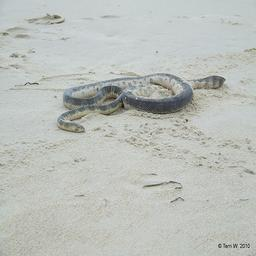
\includegraphics[width=0.4\textwidth]{ILSVRC2012_val_00000001.JPEG}
    \qquad
    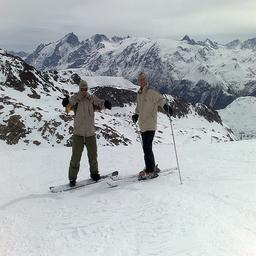
\includegraphics[width=0.4\textwidth]{ILSVRC2012_val_00000002.JPEG}
    \caption{2 Figures from ImageNet}%
    \label{fig:ImageNetExamples}%
\end{figure}

For weather dataset, it contains 10,000 images for two categories evenly, cloudy and sunny. They are from three sources, Sun Dataset\citep{russell2008labelme}, Labelme Dataset\citep{xiao2010sun} and Flickr. They were classified manually and similar images are removed. There are no unambiguous images.
\graphicspath{ {./Figures/} }
\begin{figure}[!htb]
    \centering
	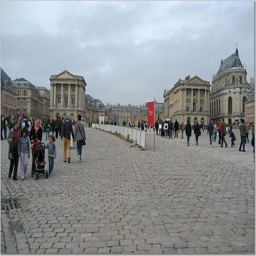
\includegraphics[width=0.4\textwidth]{cloudy_0001.png}
    \qquad
    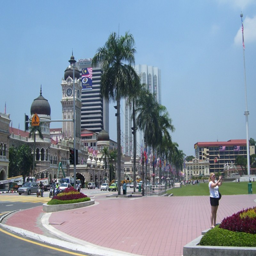
\includegraphics[width=0.4\textwidth]{sunny_0003.png}
    \caption{2 Figures from Weather Dataset}%
    \label{fig:WeatherExamples}%
\end{figure}

The two datasets are different. ImageNet dataset is for object classification and weather dataset is for scenes classification.


\section{Convolutional Neural Networks Architecture}

Due to the significant performance of AlexNet \citep{krizhevsky2012imagenet} deep convolutional neural networks, we train a model based on it. 

